\section{Results}
\label{sec:htoinv_results}

The fits of signal and background to the observed data are performed as outlined in the previous section. In the following subsections, the results of the fits for each category and data taking period are shown in several forms: pre-fit vs. post-fit distributions in each subcategory and \ptmiss bin; the observed upper limit on the signal strength parameter $\BRHinvFull$ at 95\,\% confidence level from the signal plus background hypothesis, accompanied by the median expected limit with 68\,\% and 95\,\% confidence level intervals from the background-only hypothesis; and profile likelihood ratios as a function of the signal strength.


%=========================================================


\subsection{Results of the \texorpdfstring{\ttH}{ttH} analysis}
\label{subsec:htoinv_analysis_ttH}

The \singlePhotonCr \gls{CR} is not used in constraining the \ztonunu prediction for any of the subcategories. To predict the \acrshort{qcd} event counts in the signal region, Eq.~\ref{eq:qcd_prediction} incorporates the \acrshort{mc} counts in said region and from the loose double sideband from Tab.~\ref{tab:sideband_defs_ttH}---the most enriched in multijet \acrshort{mc}. The category and \ptmiss fractions, $N_{\mathrm{SB}}^{\mathrm{QCD}}$, and $\transfac_{\mathrm{QCD}}$ were derived from the sideband.

Distributions of the post-fit yields in the signal region for 2016, 2017, and 2018 are displayed in Fig.~\ref{fig:htoinv_mountain_range_ttH_SR}. The total pre-fit background is also overlaid. Corresponding figures for the \glspl{CR} are given in App.~\ref{sec:pre_post_fit_plots_ttH_CRs}.

\begin{figure}[htbp]
    \centering
    \begin{subfigure}[b]{0.9\textwidth}
        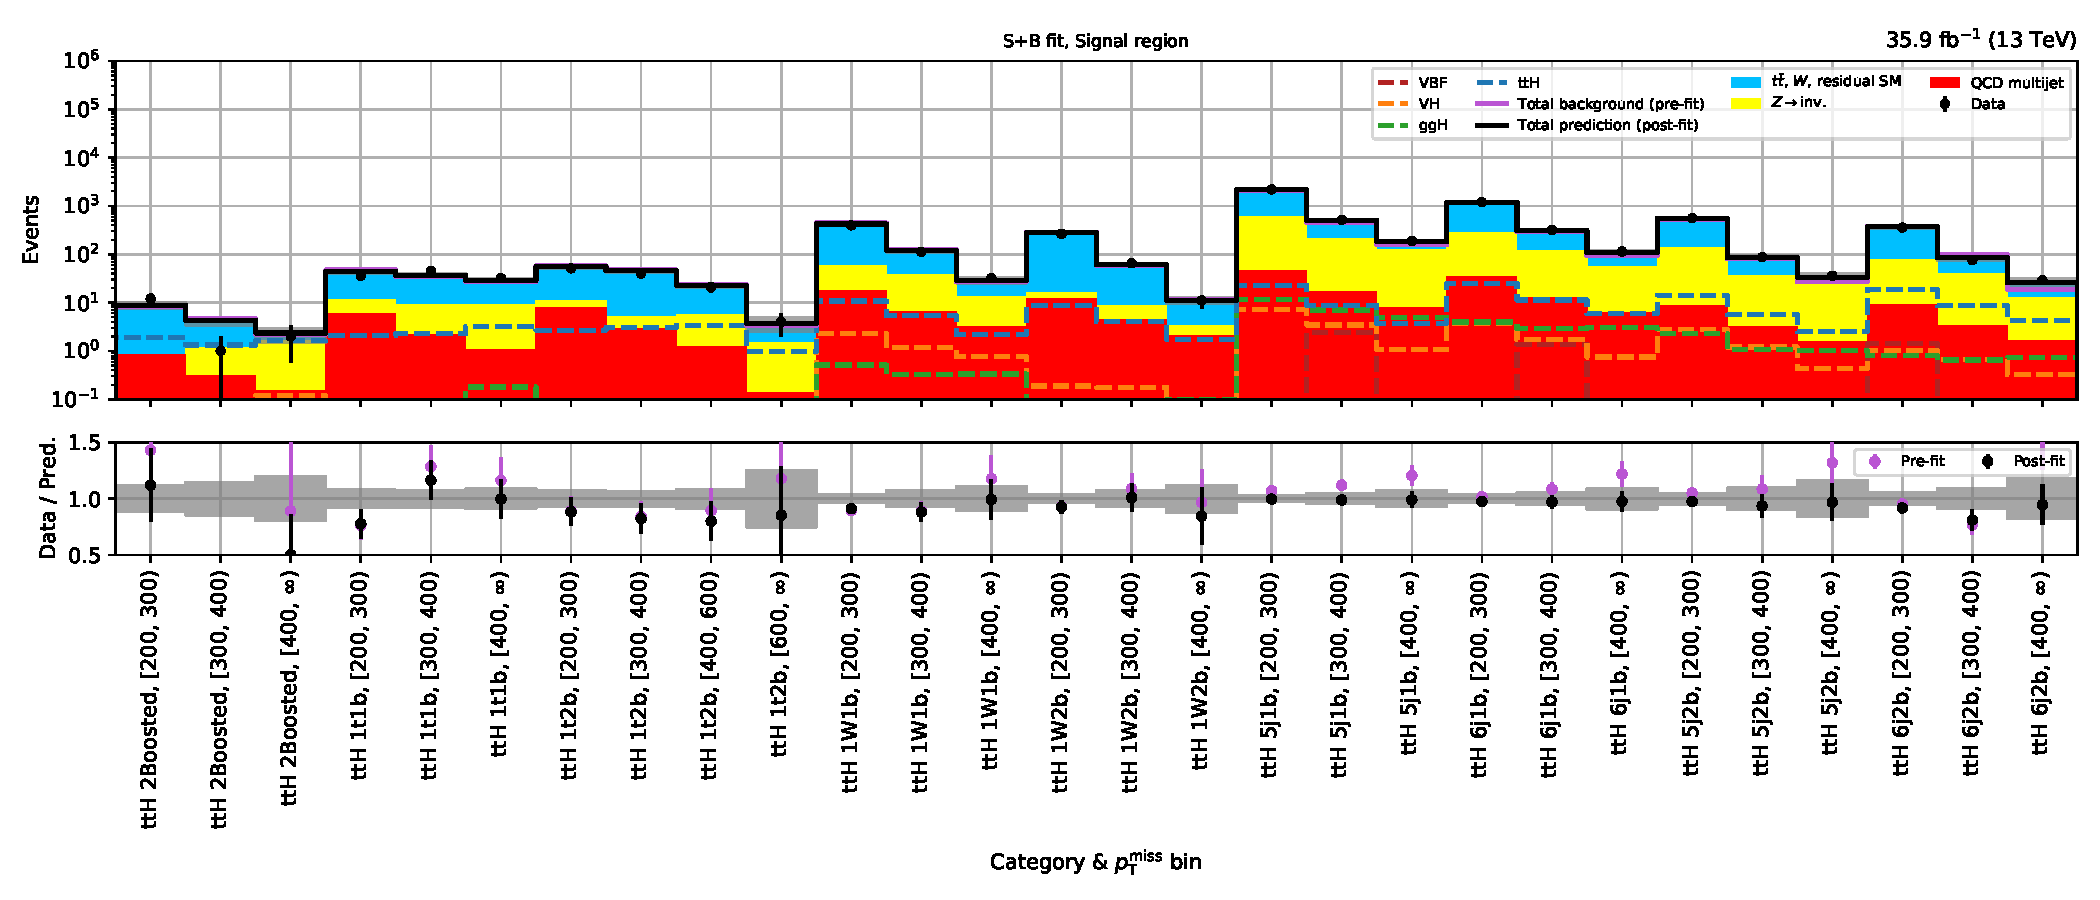
\includegraphics[width=\textwidth]{figures/mountain_ranges/2016/ttH/SR_tree_fit_s-abs_values_ttH_cats.pdf}
        \caption{\ttH --- 2016}
    \end{subfigure}

    \begin{subfigure}[b]{0.9\textwidth}
        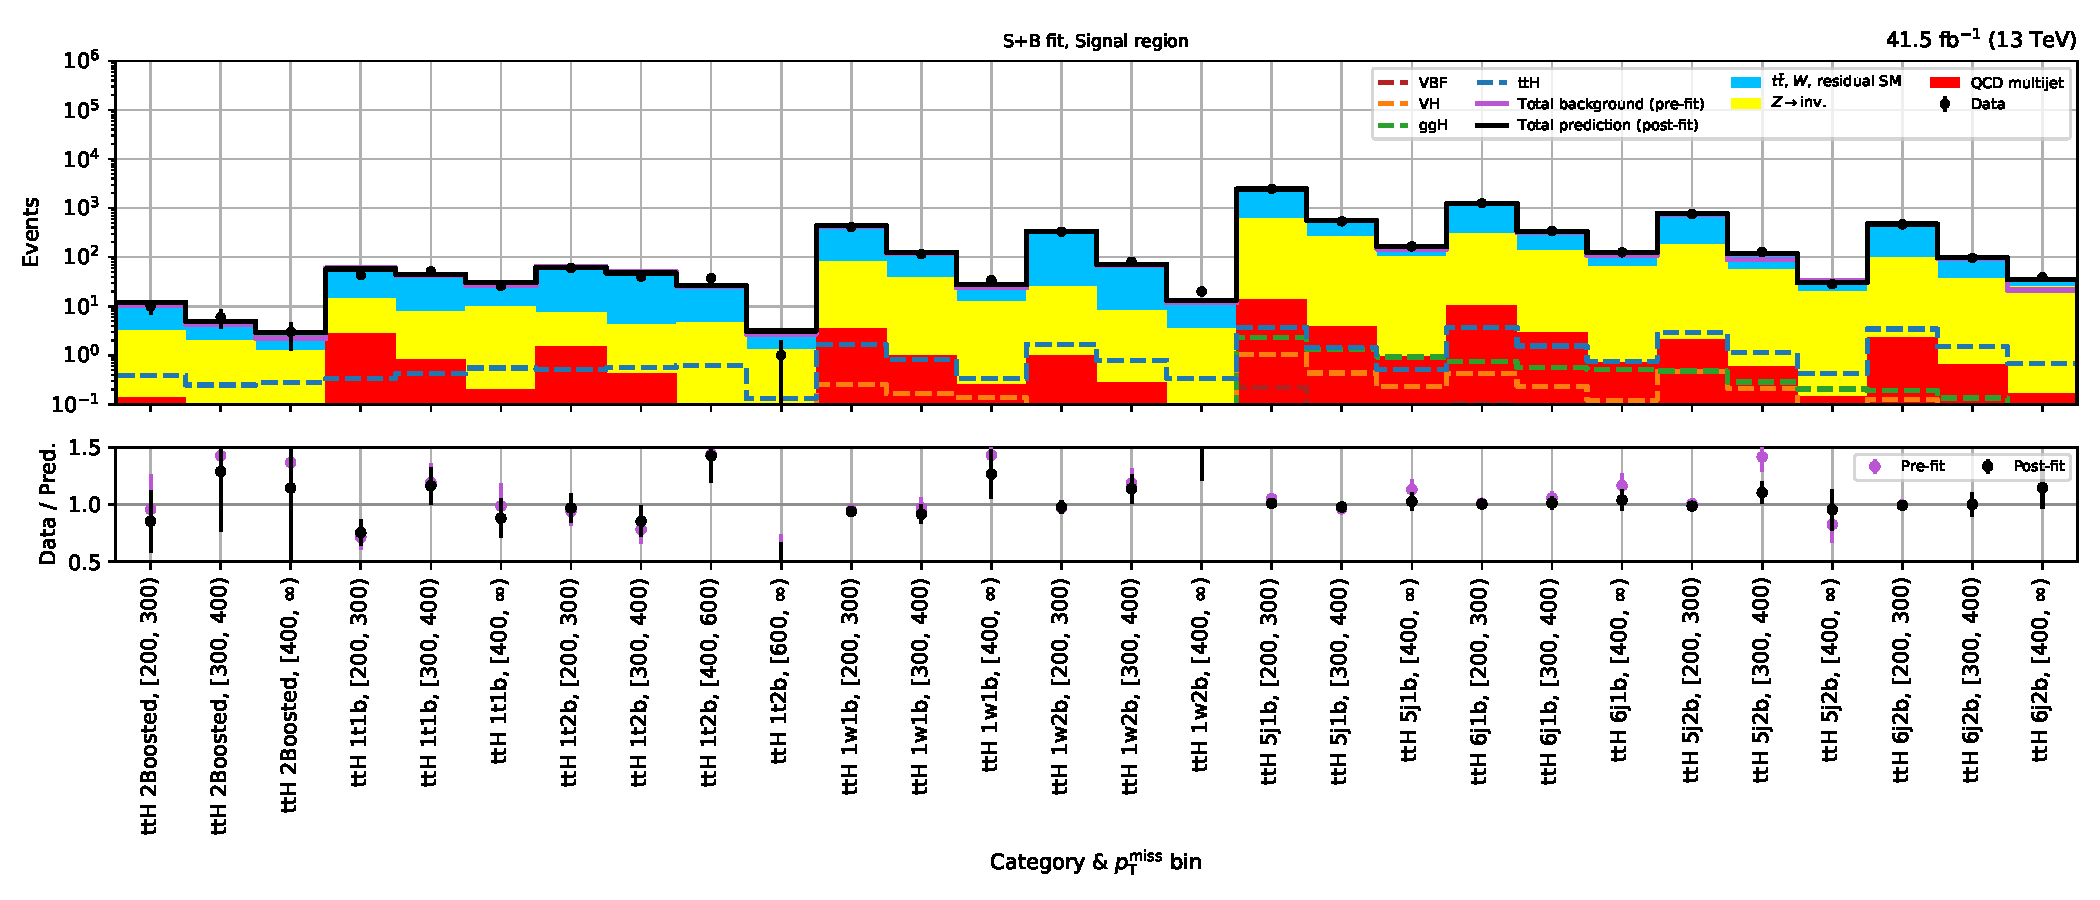
\includegraphics[width=\textwidth]{figures/mountain_ranges/2017/ttH/SR_tree_fit_s-abs_values_ttH_cats.pdf}
        \caption{\ttH --- 2017}
    \end{subfigure}

    \begin{subfigure}[b]{0.9\textwidth}
        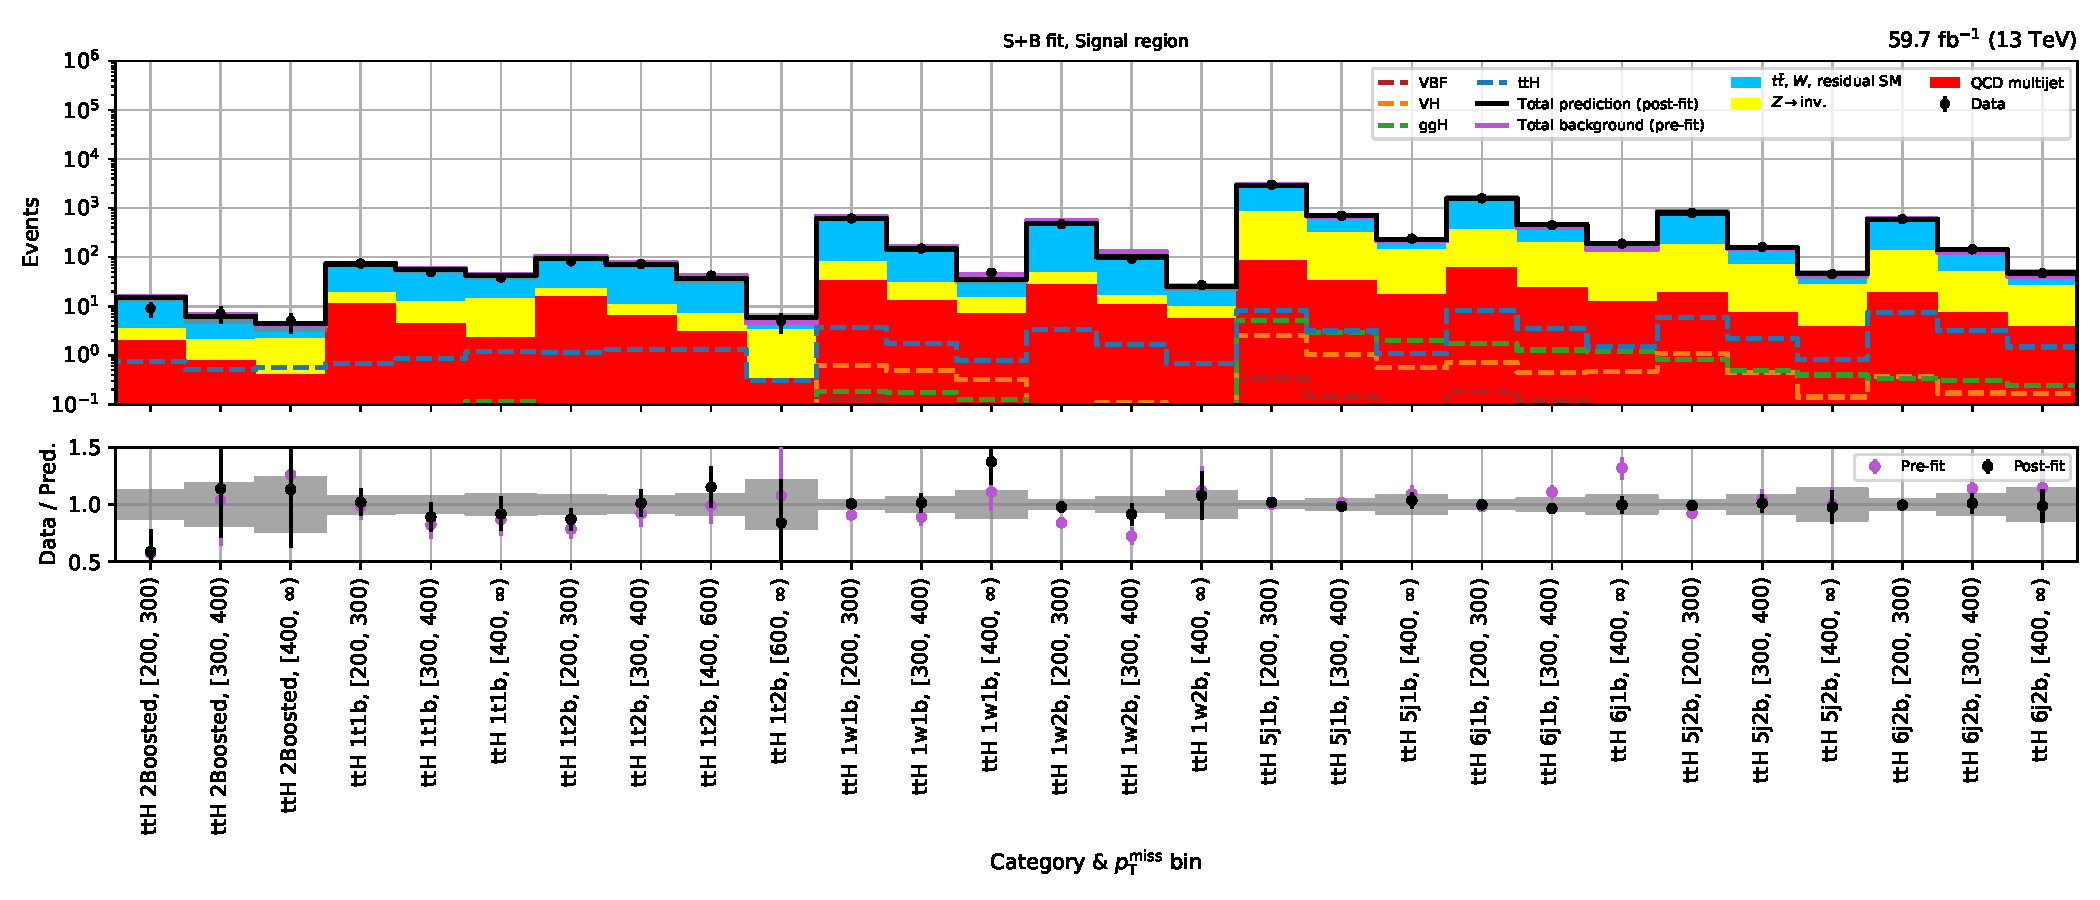
\includegraphics[width=\textwidth]{figures/mountain_ranges/2018/ttH/SR_tree_fit_s-abs_values_ttH_cats.pdf}
        \caption{\ttH --- 2018}
    \end{subfigure}
    \caption[Pre-fit and post-fit yields in the signal region for each \ttH subcategory and \ptmiss bin in each year of Run-2]{Pre-fit and post-fit yields in the signal region for each \ttH subcategory and \ptmiss bin in each year of Run-2.}
    \label{fig:htoinv_mountain_range_ttH_SR}
\end{figure}

It is evident from the distributions that the fit succeeds in most cases to match the signal and background to the data within uncertainties. Relatively few bins contain a post-fit data/prediction ratio largely different from unity. Large deviations are seen only in the \ttH boosted subcategories which are statistically limited. In 2016, a general over-prediction of background is seen, corrected for most part by the fit. The pre-fit ratio is overall better in 2016 than in the other years. The effect of pre-firing was less severe than in 2017. Both of the later years suffered from additional problems such as noise in the \acrshort{ecal} end caps in 2017---affecting \ttH given its high jet multiplicity---and the HEM issue in 2018 that largely affects \glspl{jet}. Techniques were employed to mitigate the problems, but of course may have failed to completely eradicate them.

\acrshort{qcd} multijet is a somewhat large background in several of the subcategories despite the \mindphi, \omegaTilde, and \gls{bjet}/boosted object requirements. Even though they are designed to reject a significant of the multijet background, the high cross section of the process and prevalence for mismeasurement necessitates accurate modelling.

These post-fit distributions translate directly into the upper limit on \BRHinvFull. Fig.~\ref{fig:htoinv_limit_ttH} showcases the limit and profile likelihood scan for the \ttH category in each data taking year individually and the combination over the full Run-2 dataset. Limits broken down by subcategory in each year are presented in Fig.~\ref{fig:htoinv_limit_ttH_per_year}.

\begin{figure}[htbp]
    \centering
    \begin{subfigure}[t]{0.45\textwidth}
        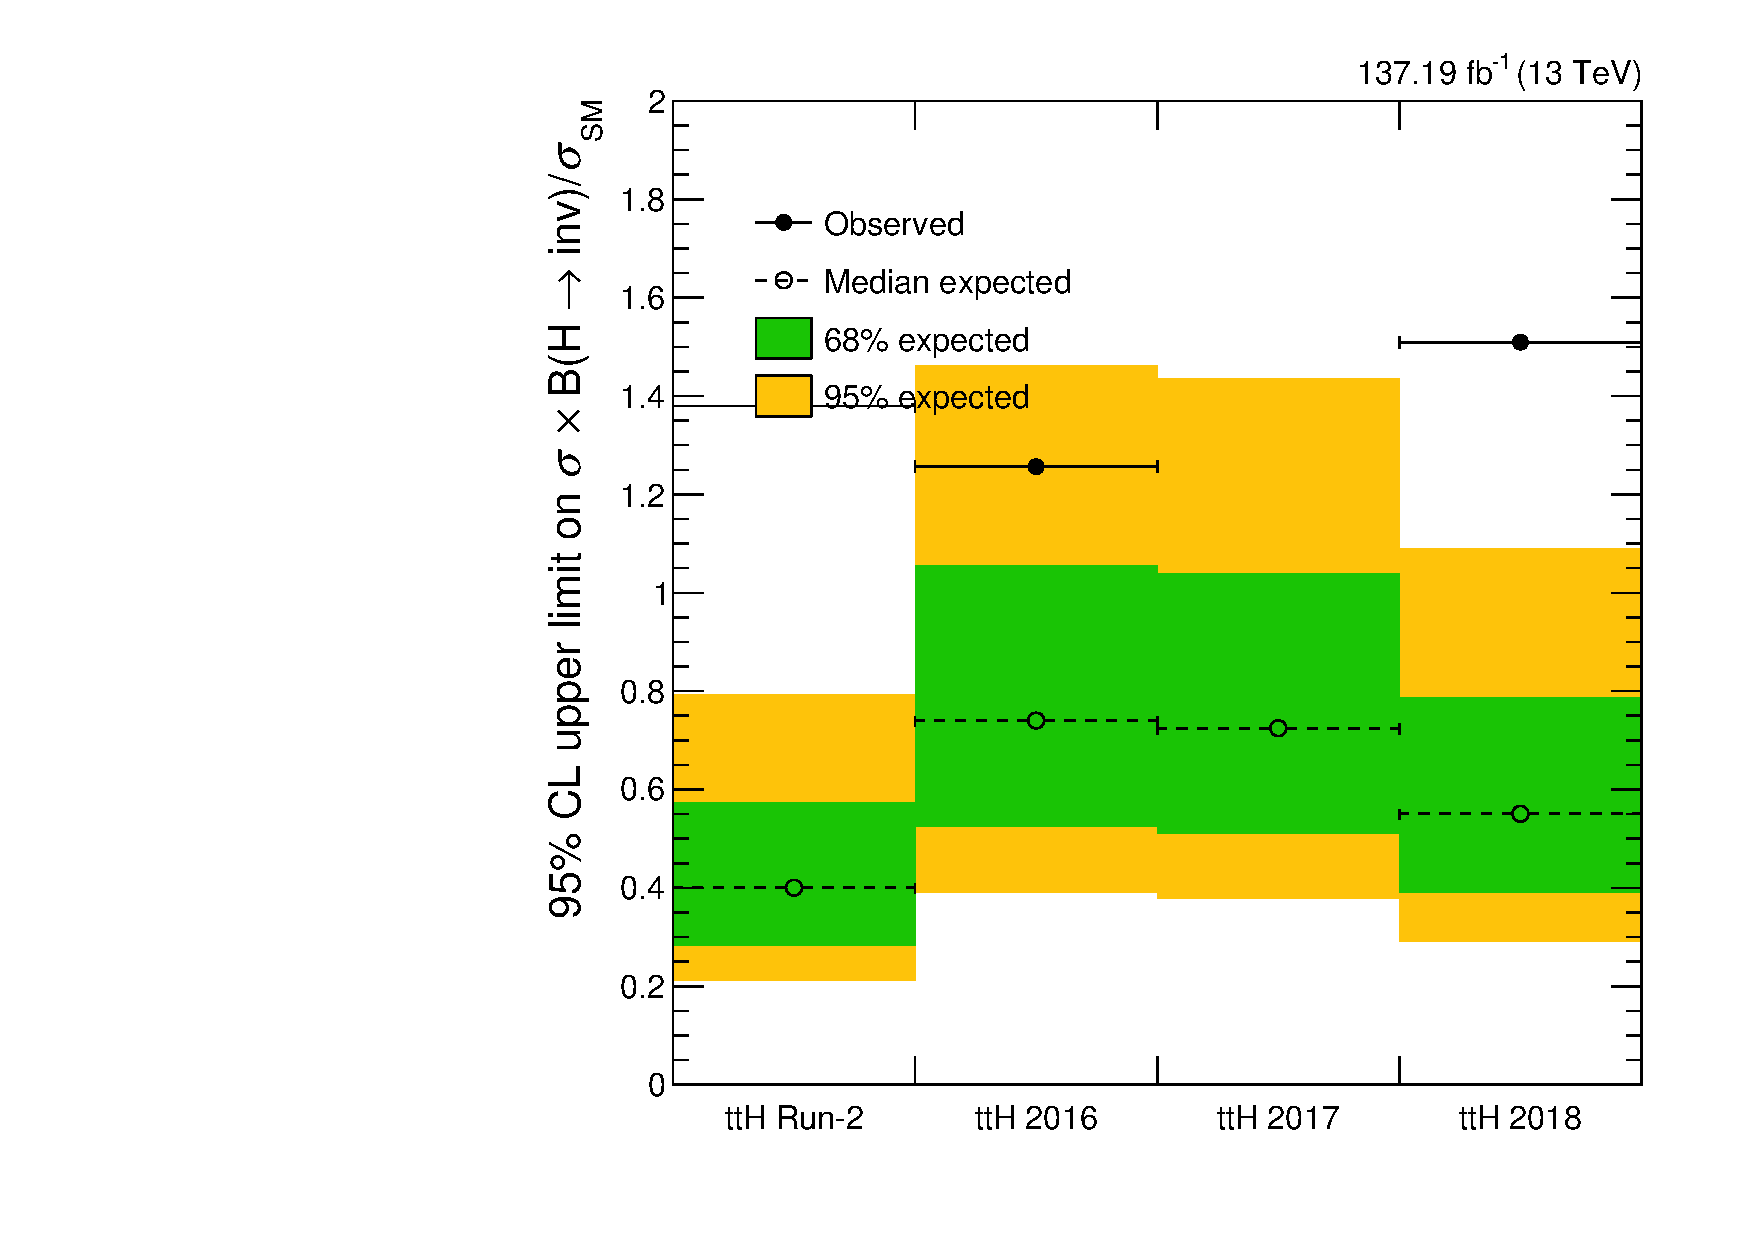
\includegraphics[width=\textwidth]{figures/limits/ttH/limit_Run2_ttH.pdf}
        \caption{Limit --- \ttH}
    \end{subfigure}
    \hspace{0.05\textwidth}
    \begin{subfigure}[t]{0.45\textwidth}
        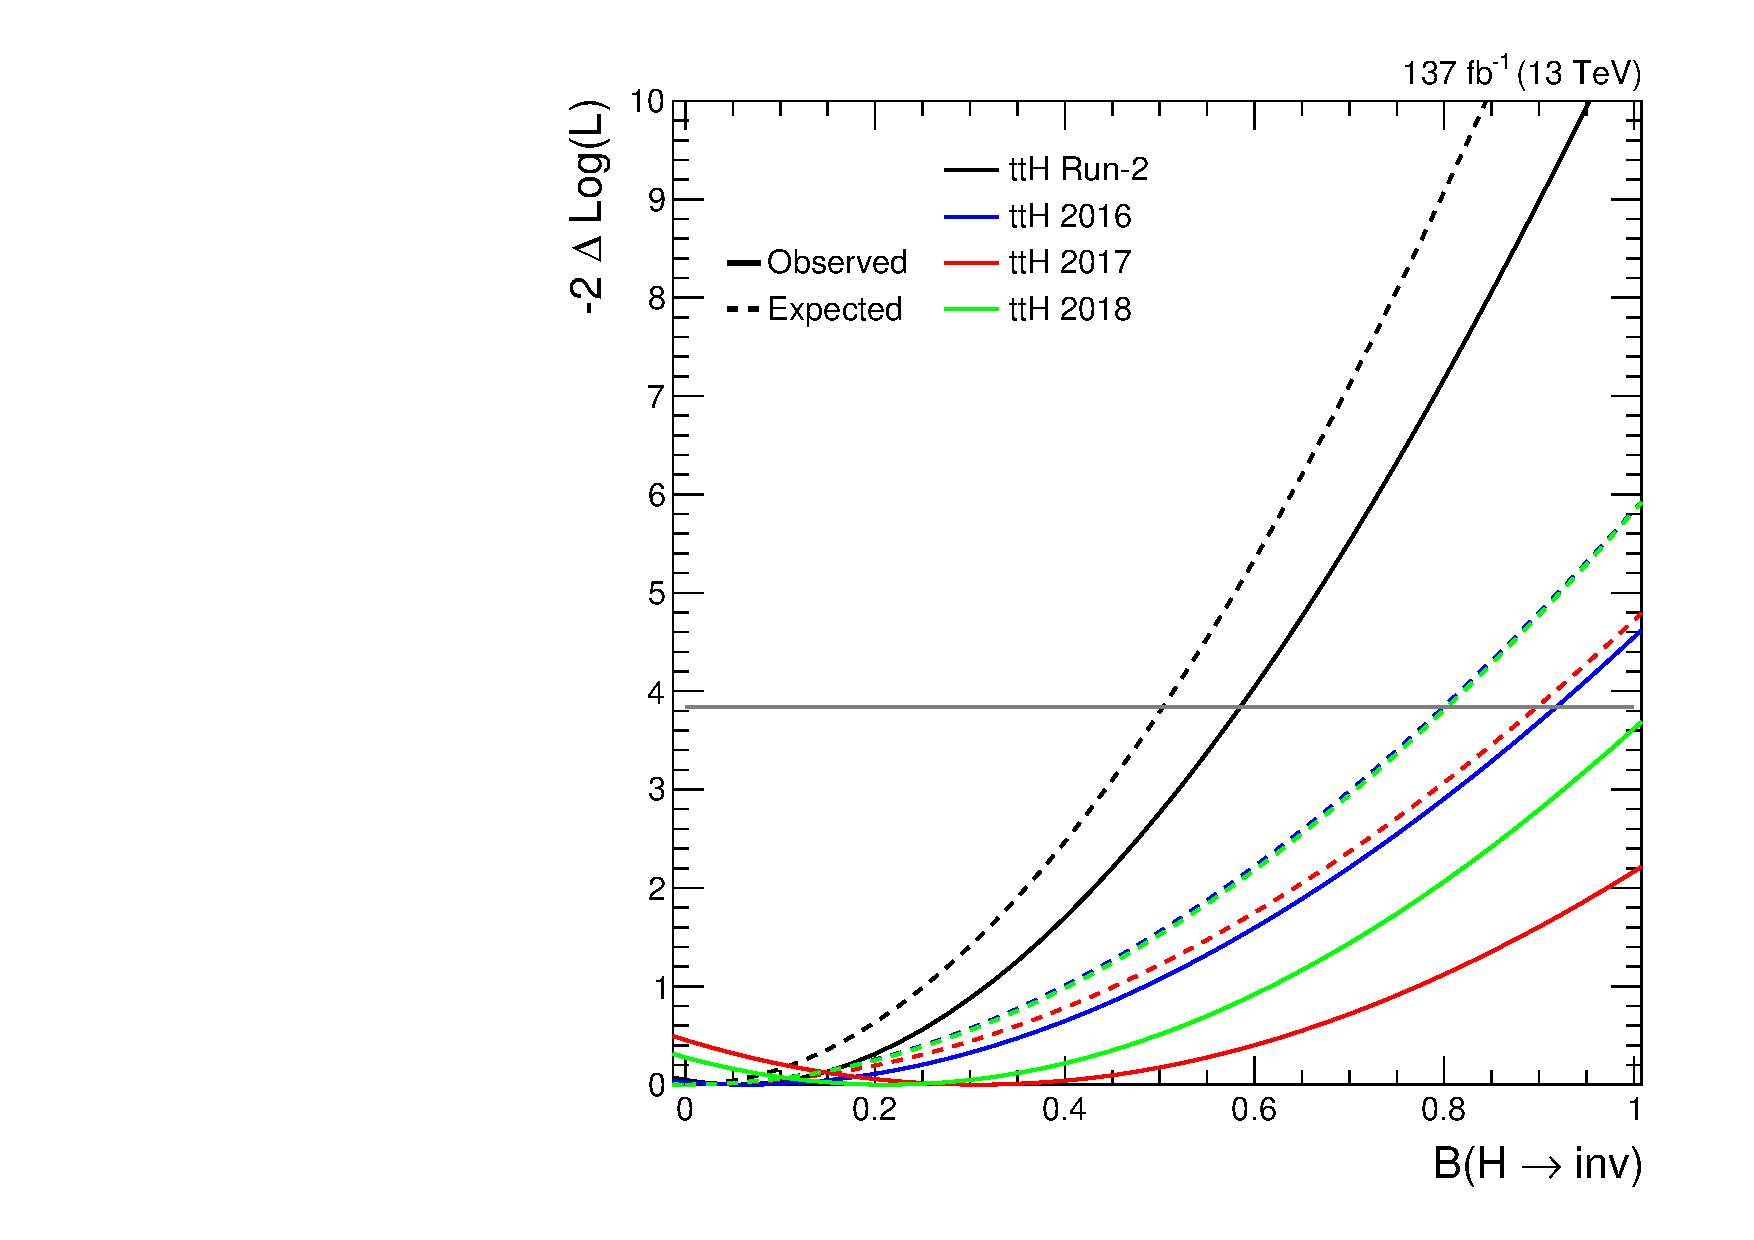
\includegraphics[width=\textwidth]{figures/likelihood_scan/profile_likelihood_scan_Run2_ttH.pdf}
        \caption{Profile likelihood --- \ttH}
    \end{subfigure}
    \caption[Observed and expected 95\,\% CL upper limit on the Higgs boson to invisible state branching fraction $\BRof{\higgstoinv}$ (left) and the corresponding profile likelihood ratio as a function of it (right) in the \ttH category]{Observed and expected 95\,\% CL upper limit on the Higgs boson to invisible state branching fraction $\BRof{\higgstoinv}$ (left) and the corresponding profile likelihood ratio as a function of it (right) in the \ttH category. The result from each data taking period is presented along with their combination.}
    \label{fig:htoinv_limit_ttH}
\end{figure}

The limits are reasonably consistent between years with similar values and the observed slightly higher than the median expectation; a feature also seen in the combination. The combined Run-2 limit of 50\,\% expected and 56\,\% observed is significantly more sensitive than the analogous combination from \acrshort{atlas} of 94\,\% observed and 64\,\% expected~\cite{Aad:2020sgw}. A comparison the 2016 result from \acrshort{cms} show very similar sensitivity, with 85\,\% observed and 73\,\% expected in the 0-lepton channel~\cite{CMS-PAS-HIG-18-008}. The better sensitivity in the published could be explained by a number of reasons. Additional systematic uncertainties were included in this result that are not present in the published one such as the \acrshort{qcd} scale for top quark processes, \acrlong{jer}, or those associated with the \acrshort{nlo} corrections to $\PVec \plusjets$ backgrounds.

By subcategory, those targeting the boosted topologies are the most sensitive to the invisible decays of the Higgs boson. Given the purity of these subcategories, it is understandable why. The signal-to-background ratio is much higher, as evident from the post-fit distributions. However, statistical and systematic uncertainties could have a larger relative effect than in resolved-targeting subcategories. These give generally weaker limits than the boosted subcategories, but with greater statistical power, typically lead to smaller uncertainties surrounding the limits. The sensitivity landscape is mostly consistent between years, more so for 2017 and 2018 given the similarities in simulation and detector configuration. All of the observations are within the $\text{2}\sigma$ boundaries of the expected limit, with many within $\text{1}\sigma$, demonstrating a consistent picture between background and data.

The profile likelihood scan illustrates how the likelihood function for the fit over a set of subcategories evolves with the upper limit on branching ratio. The horizontal line $-\text{2}\Delta \ln(\likelihood) = \text{3.84}$ represents the 95\,\% confidence level. It can therefore be seen that the intersection of a dashed curve with the line is equal to the median expected limit and the intersection of a solid curve equals the measured observed limit. Indicative of the stability and health of the fit, the likelihood scans in Fig.~\ref{fig:htoinv_limit_ttH} are satisfactory with minima near $\BR = \text{0}$, rising smoothly either side of it.

\clearpage


%=========================================================


\subsection{Results of the \texorpdfstring{\VH}{VH} analysis}
\label{subsec:htoinv_analysis_VH}

Contrary to \ttH, all of the \glspl{CR} are utilised in the non-multijet background predictions. A more accurate \ztonunu prediction is possible since it can be constrained by three \glspl{CR}. The single sideband inverted in \mindphi, \omegaTilde, and dijet mass was applied to predict the \acrshort{qcd} contribution to the signal region in all \VH subcategories.

Distributions of the pre-fit and post-fit yields for 2016, 2017, and 2018 are displayed in Fig.~\ref{fig:htoinv_mountain_range_VH_SR}. Corresponding figures for the \glspl{CR} are given in App.~\ref{sec:pre_post_fit_plots_VH_CRs}.

\begin{figure}[htbp]
    \centering
    \begin{subfigure}[b]{0.9\textwidth}
        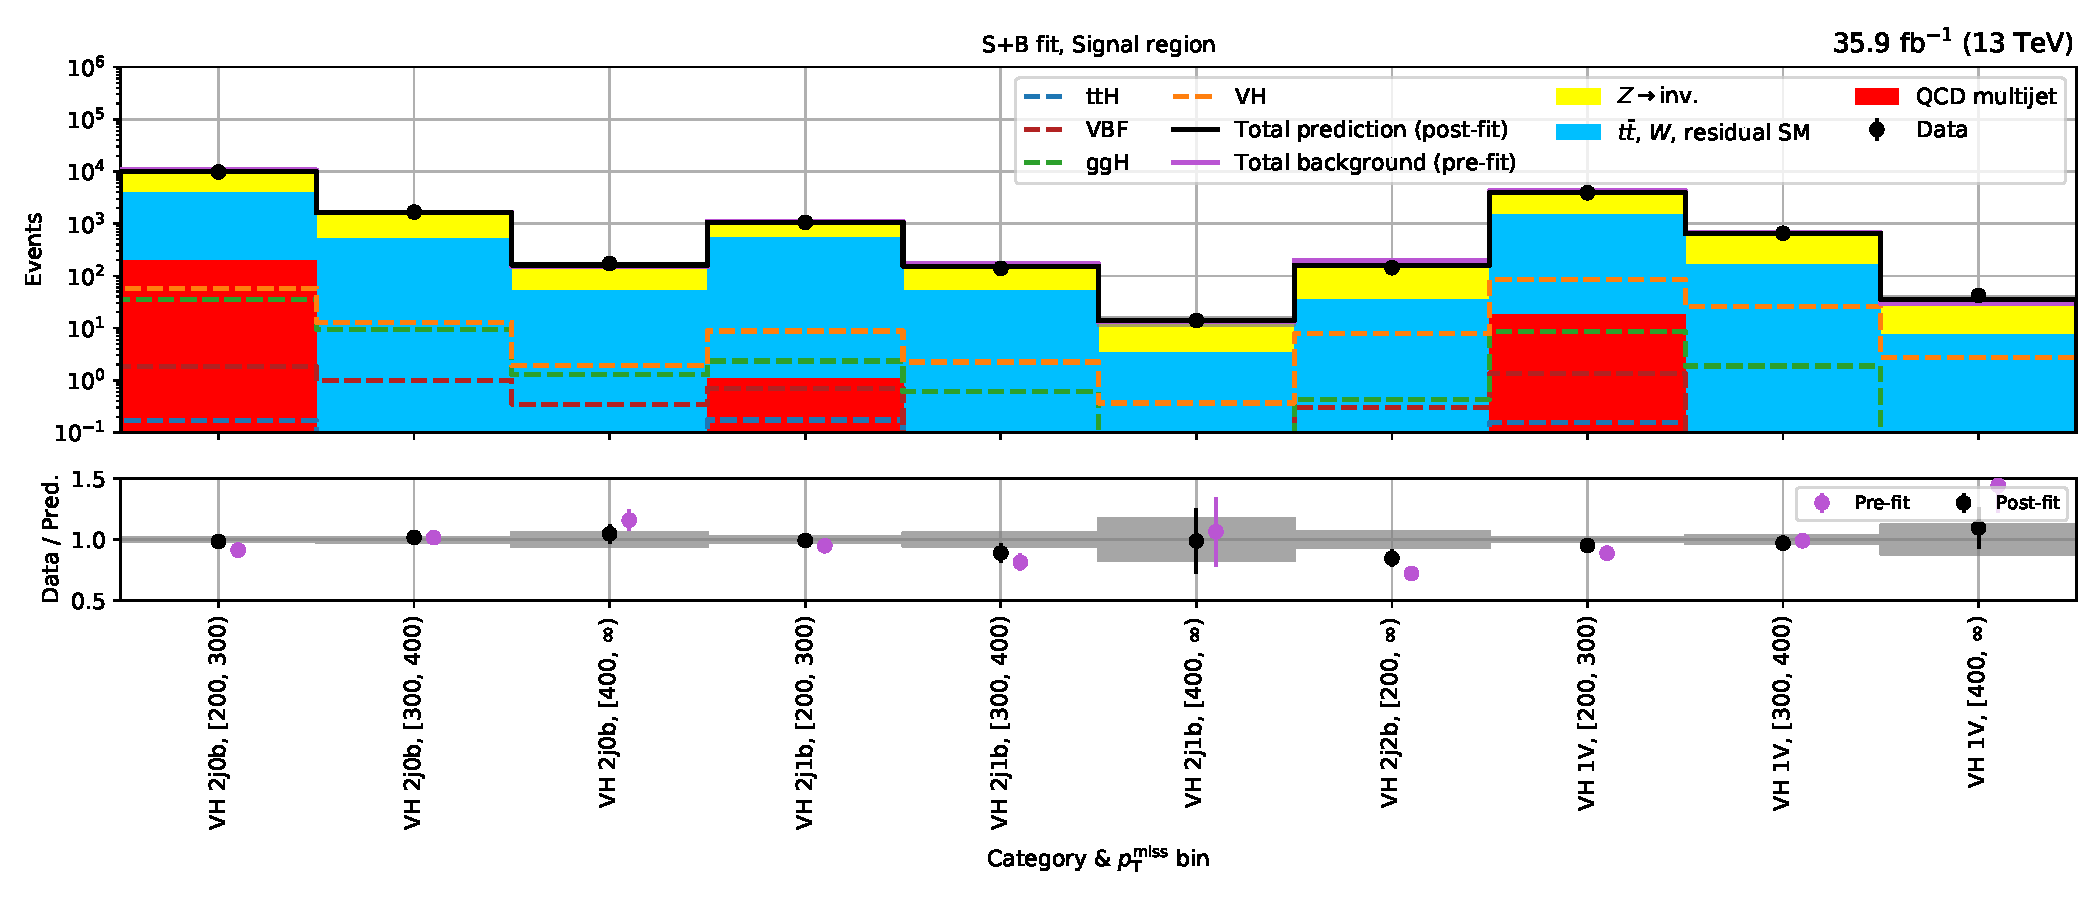
\includegraphics[width=\textwidth]{figures/mountain_ranges/2016/VH/SR_tree_fit_s-abs_values_VH_cats.pdf}
        \caption{\VH --- 2016}
    \end{subfigure}

    \begin{subfigure}[b]{0.9\textwidth}
        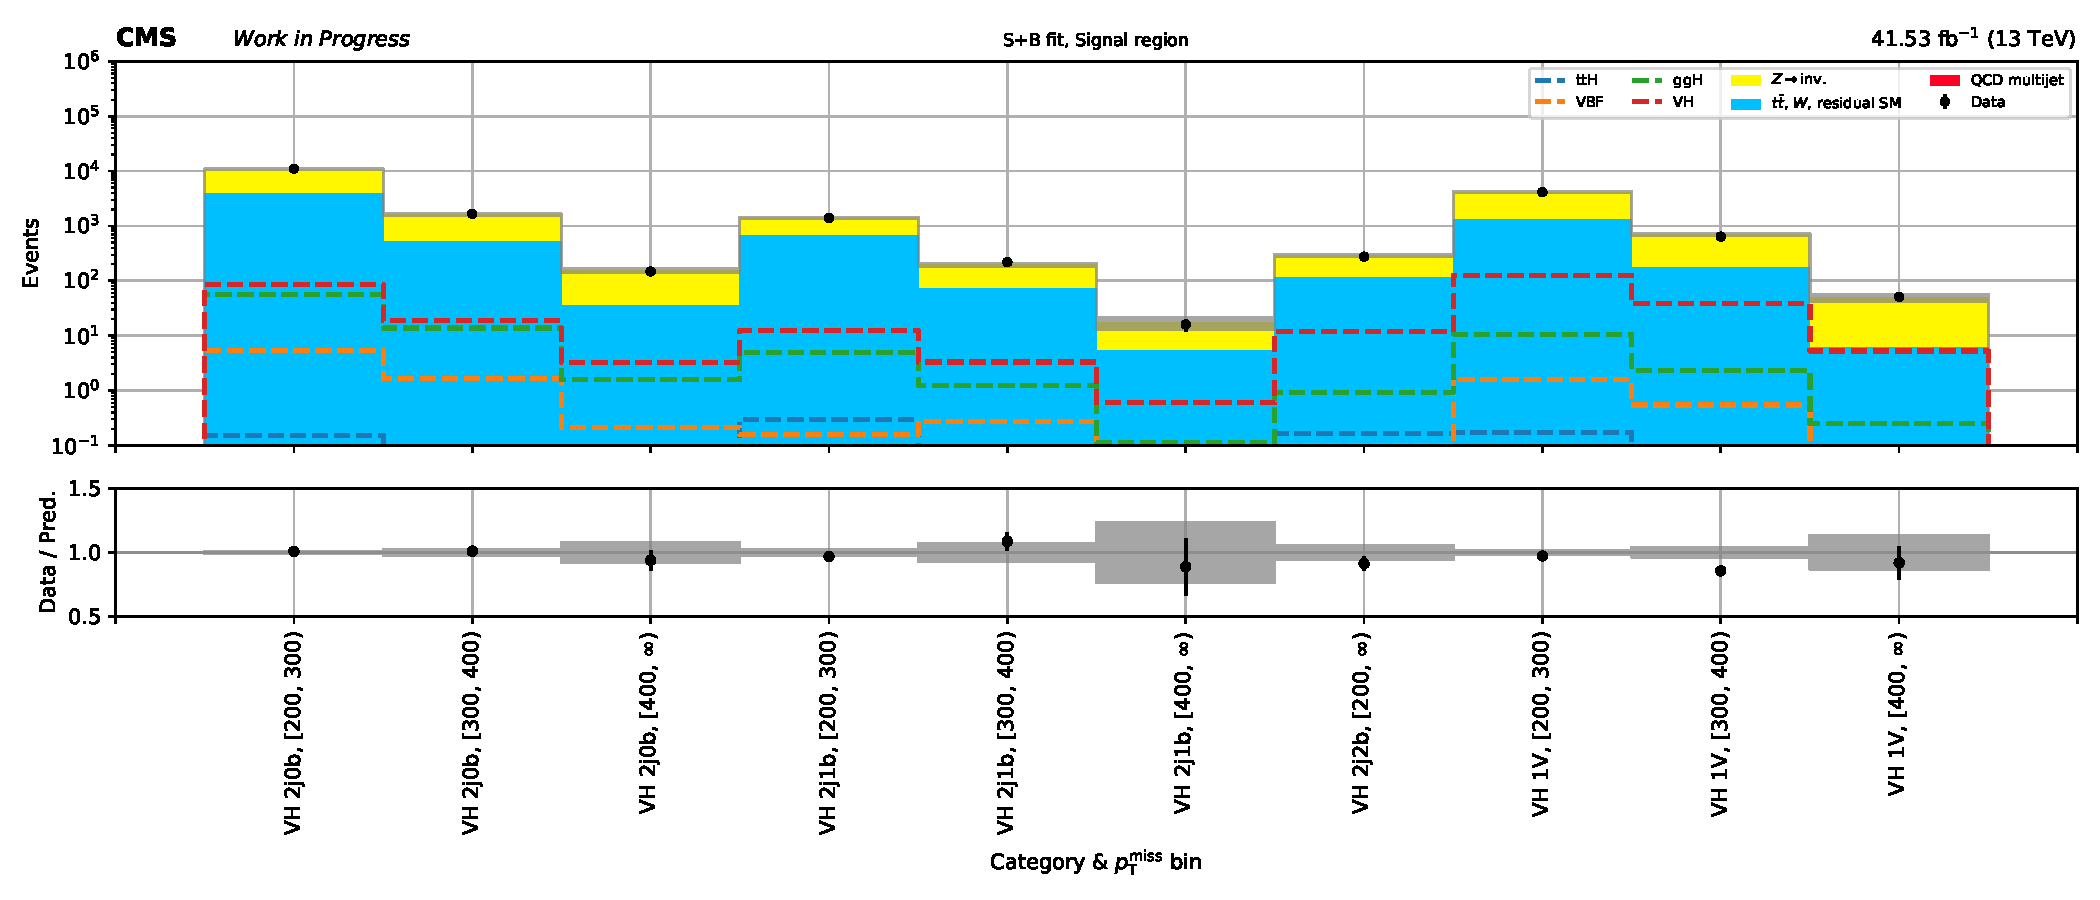
\includegraphics[width=\textwidth]{figures/mountain_ranges/2017/VH/SR_tree_fit_s-abs_values_VH_cats.pdf}
        \caption{\VH --- 2017}
    \end{subfigure}

    \begin{subfigure}[b]{0.9\textwidth}
        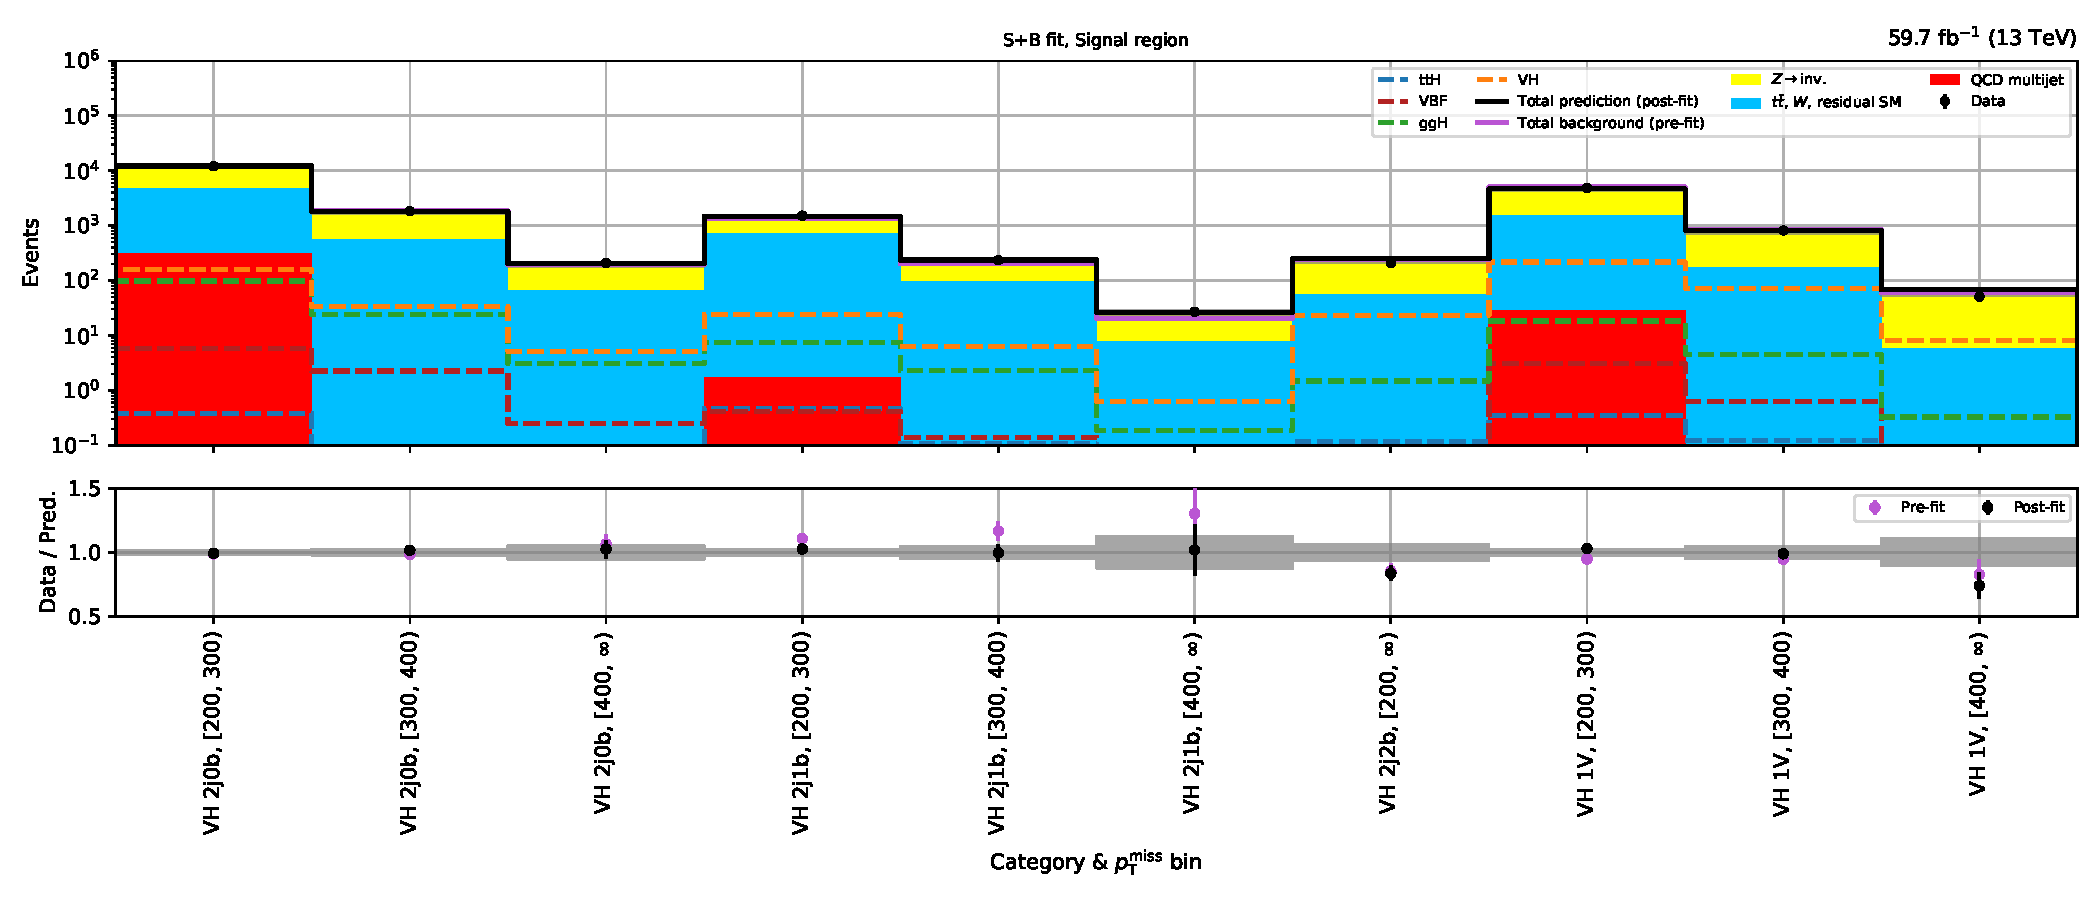
\includegraphics[width=\textwidth]{figures/mountain_ranges/2018/VH/SR_tree_fit_s-abs_values_VH_cats.pdf}
        \caption{\VH --- 2018}
    \end{subfigure}
    \caption[Pre-fit and post-fit yields in the signal region for each \VH subcategory and \ptmiss bin in each year of Run-2]{Pre-fit and post-fit yields in the signal region for each \VH subcategory and \ptmiss bin in each year of Run-2.}
    \label{fig:htoinv_mountain_range_VH_SR}
\end{figure}

The \VH topology is dominated by the irreducible \ztonunupjets background, followed by lost lepton, and finally a small amount of \acrshort{qcd} multijet. Especially with the \gls{bjet}/boosted object requirements, and dijet signature coupled to a small mass window around the electroweak bosons, it is a percent-level background in the bins it appears in. The post-fit prediction agrees with the data very well in most cases, demonstrating adequate background predictions and leaving little room for signal to be inflated.

Fig.~\ref{fig:htoinv_limit_VH} showcases the expected and observed limits for the \VH category in each year and the Run-2 combination. Limits for each subcategory can be found in Fig.~\ref{fig:htoinv_limit_VH_per_year}.

\begin{figure}[htbp]
    \centering
    \begin{subfigure}[t]{0.45\textwidth}
        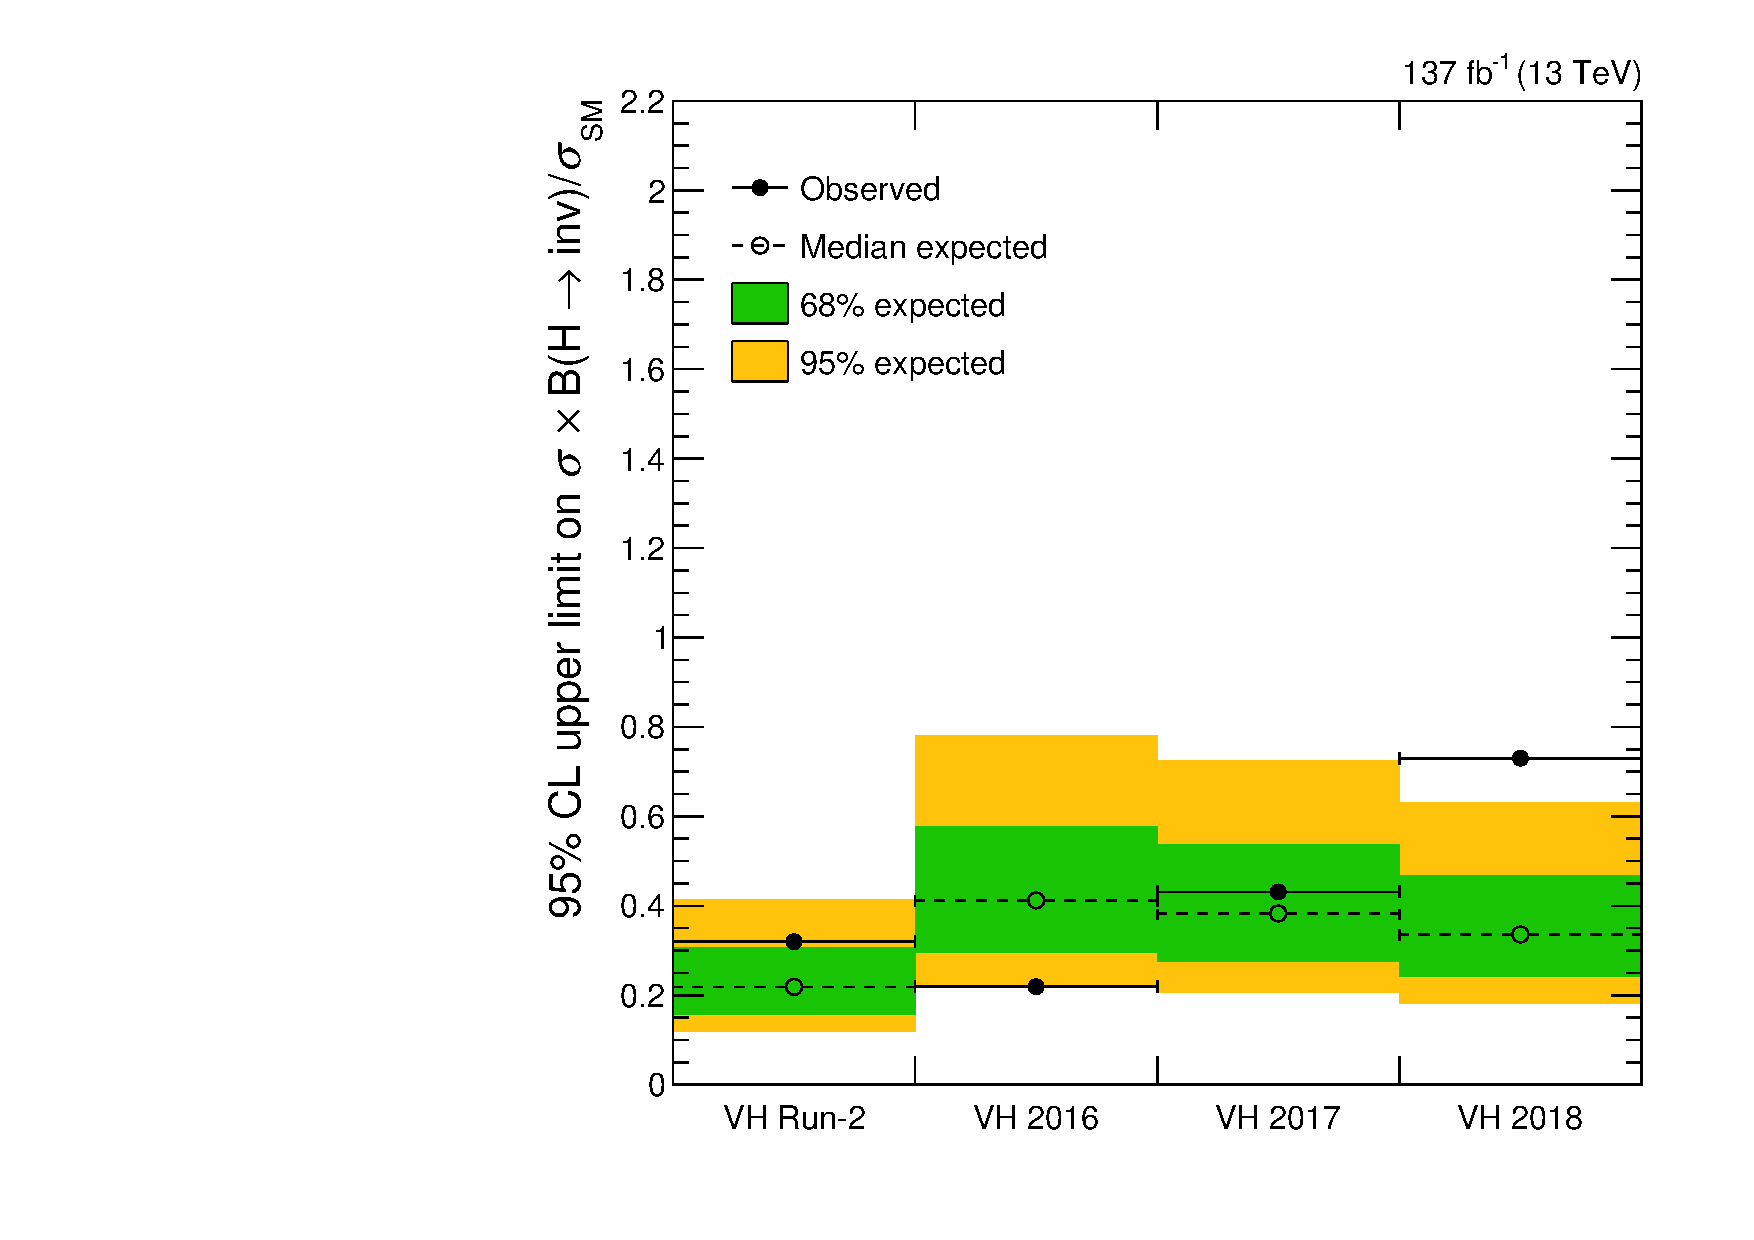
\includegraphics[width=\textwidth]{figures/limits/VH/limit_Run2_VH.pdf}
        \caption{Limit --- \VH}
    \end{subfigure}
    \hspace{0.05\textwidth}
    \begin{subfigure}[t]{0.45\textwidth}
        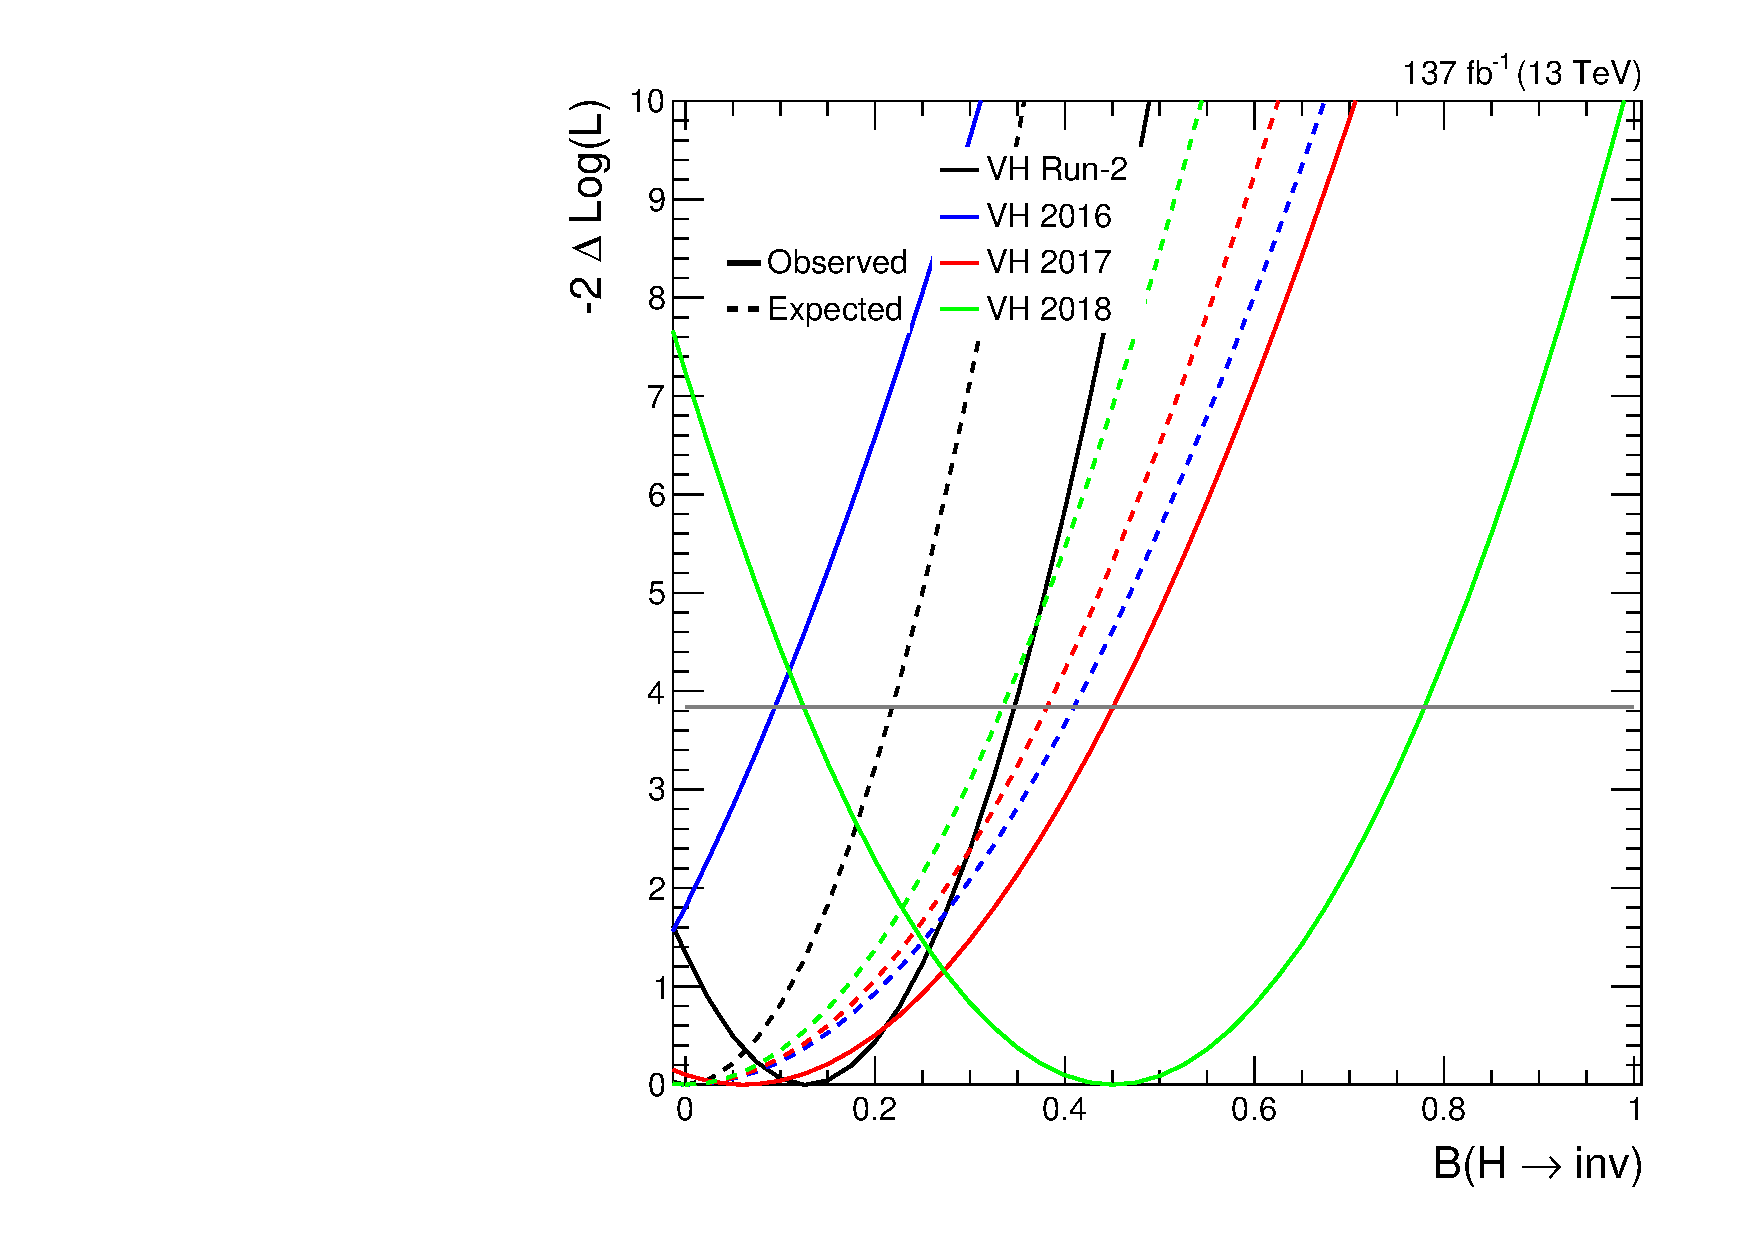
\includegraphics[width=\textwidth]{figures/likelihood_scan/profile_likelihood_scan_Run2_VH.pdf}
        \caption{Profile likelihood --- \VH}
    \end{subfigure}
    \caption[Observed and expected 95\,\% CL upper limit on the Higgs boson to invisible state branching fraction $\BRof{\higgstoinv}$ (left) and the corresponding profile likelihood ratio as a function of it (right) in the \VH category]{Observed and expected 95\,\% CL upper limit on the Higgs boson to invisible state branching fraction $\BRof{\higgstoinv}$ (left) and the corresponding profile likelihood ratio as a function of it (right) in the \VH category. The result from each data taking period is presented along with their combination.}
    \label{fig:htoinv_limit_VH}
\end{figure}

The obtained limits demonstrate that the sensitivity of the \VH topology to \higgstoinv is second only to \acrshort{vbf}. Fig.~\ref{fig:htoinv_limit_VH_per_year} makes apparent that the sensitivity of \VH within a given year, and overall, is driven by the 1V subcategory. It is closely followed by 2j2b (targeting $\HepProcess{\PZ \to \Pqb\Paqb}$) and 2j0b (rich in $\HepProcess{\PVec \to \Pquark\APquark}$). 2j1b lags behind as it relies on a \gls{bjet} being falsely tagged or missed by the \deepcsv algorithm.

For comparisons to public results, there are no full Run-2 $\VH(\higgstoinv)$ searches or interpretations. Results from both \acrshort{atlas} and \acrshort{cms} are, however, available using 2016 data. The latter is a mono-\PVec search comparable to the 1V subcategory from this thesis. The \acrshort{atlas} \VH result found an observed limit of 83\,\% and expected of 58\,\%, while from \acrshort{cms} they were 50\,\% and 48\,\%, respectively. From this thesis, an observed limit of 67\,\% and expected of 55\,\% were obtained. Sensitivity is better than that of \acrshort{atlas} but worse than the \acrshort{cms} result. Differences in signal modelling are thought to be a factor. Older simulated signal samples have been found to use fixed factorisation scales at the \PW or \PH mass as opposed to the running scales in newer samples such as those used in this thesis. The harder Higgs boson \pt (i.e., \ptmiss) spectrum in the older samples could be responsible for an artificially greater sensitivity. If present in the \ttH sample from the 2016 public result, it may be another reason for the improved limit over those from this analysis.

% Info about signal scale from 2016: https://indico.cern.ch/event/978146/contributions/4120060/attachments/2149295/3623502/2020-11-20_monov_update%2B.pdf

The results per year in Fig.~\ref{fig:htoinv_limit_VH} are inconsistent to some degree, with an observation slightly below the $\text{2}\sigma$ boundary of the expected limit in 2016, correspondence in 2017, and an excess in 2018. In 2018, the observed limit is noticeably worse than in the preceding two. Inference from Fig.~\ref{fig:htoinv_mountain_range_VH_2018_CRs} suggests it is due the over-prediction of simulation in all of the leptonic \glspl{CR} of the 1V subcategory, consequently scaling down the background in the signal region. While not necessarily an issue in the final \ptmiss bin, it could indicate that the limit is sensitive to the agreement in the lower bins. The 2j0b observation is also outside the $\text{2}\sigma$ interval, further affecting the fit to the whole category.

\clearpage


%=========================================================


\subsection{Combined results}
\label{subsec:htoinv_combined_results}

Upper limits for $\BRof{\higgstoinv}$ by combining all categories for the full Run-2 dataset can be shown as broken down by data taking year in Fig.~\ref{fig:htoinv_limit_likelihood_Run2_per_year} and by category in Fig.~\ref{fig:htoinv_limit_likelihood_Run2_per_cat}. Profile likelihood ratios as a function of $\BRof{\higgstoinv}$ are also presented opposite the limits. Corresponding limits and likelihood ratios for each year are displayed in Figs.~\ref{fig:htoinv_limit_likelihood_2016}, \ref{fig:htoinv_limit_likelihood_2017}, \ref{fig:htoinv_limit_likelihood_2018}, respectively, of App.~\ref{sec:limits_likelihoods_year_supplementary}.\footnote{Add some reasonable discussion of the limits and likelihoods, consistency across categories/years, once I have the final results.}\footnote{If we see worse results in 2016 compared to previous analyses, one explainer could be the signal models. It was recently discovered that signal MC used for 2016 analyses had a harder pt spectrum than what has been used in this analysis, which would give improved limits there as the distributions are shifted to higher MET and giving better signal sensitivity.}

\begin{figure}[htbp]
    \centering
    \begin{subfigure}[t]{0.45\textwidth}
        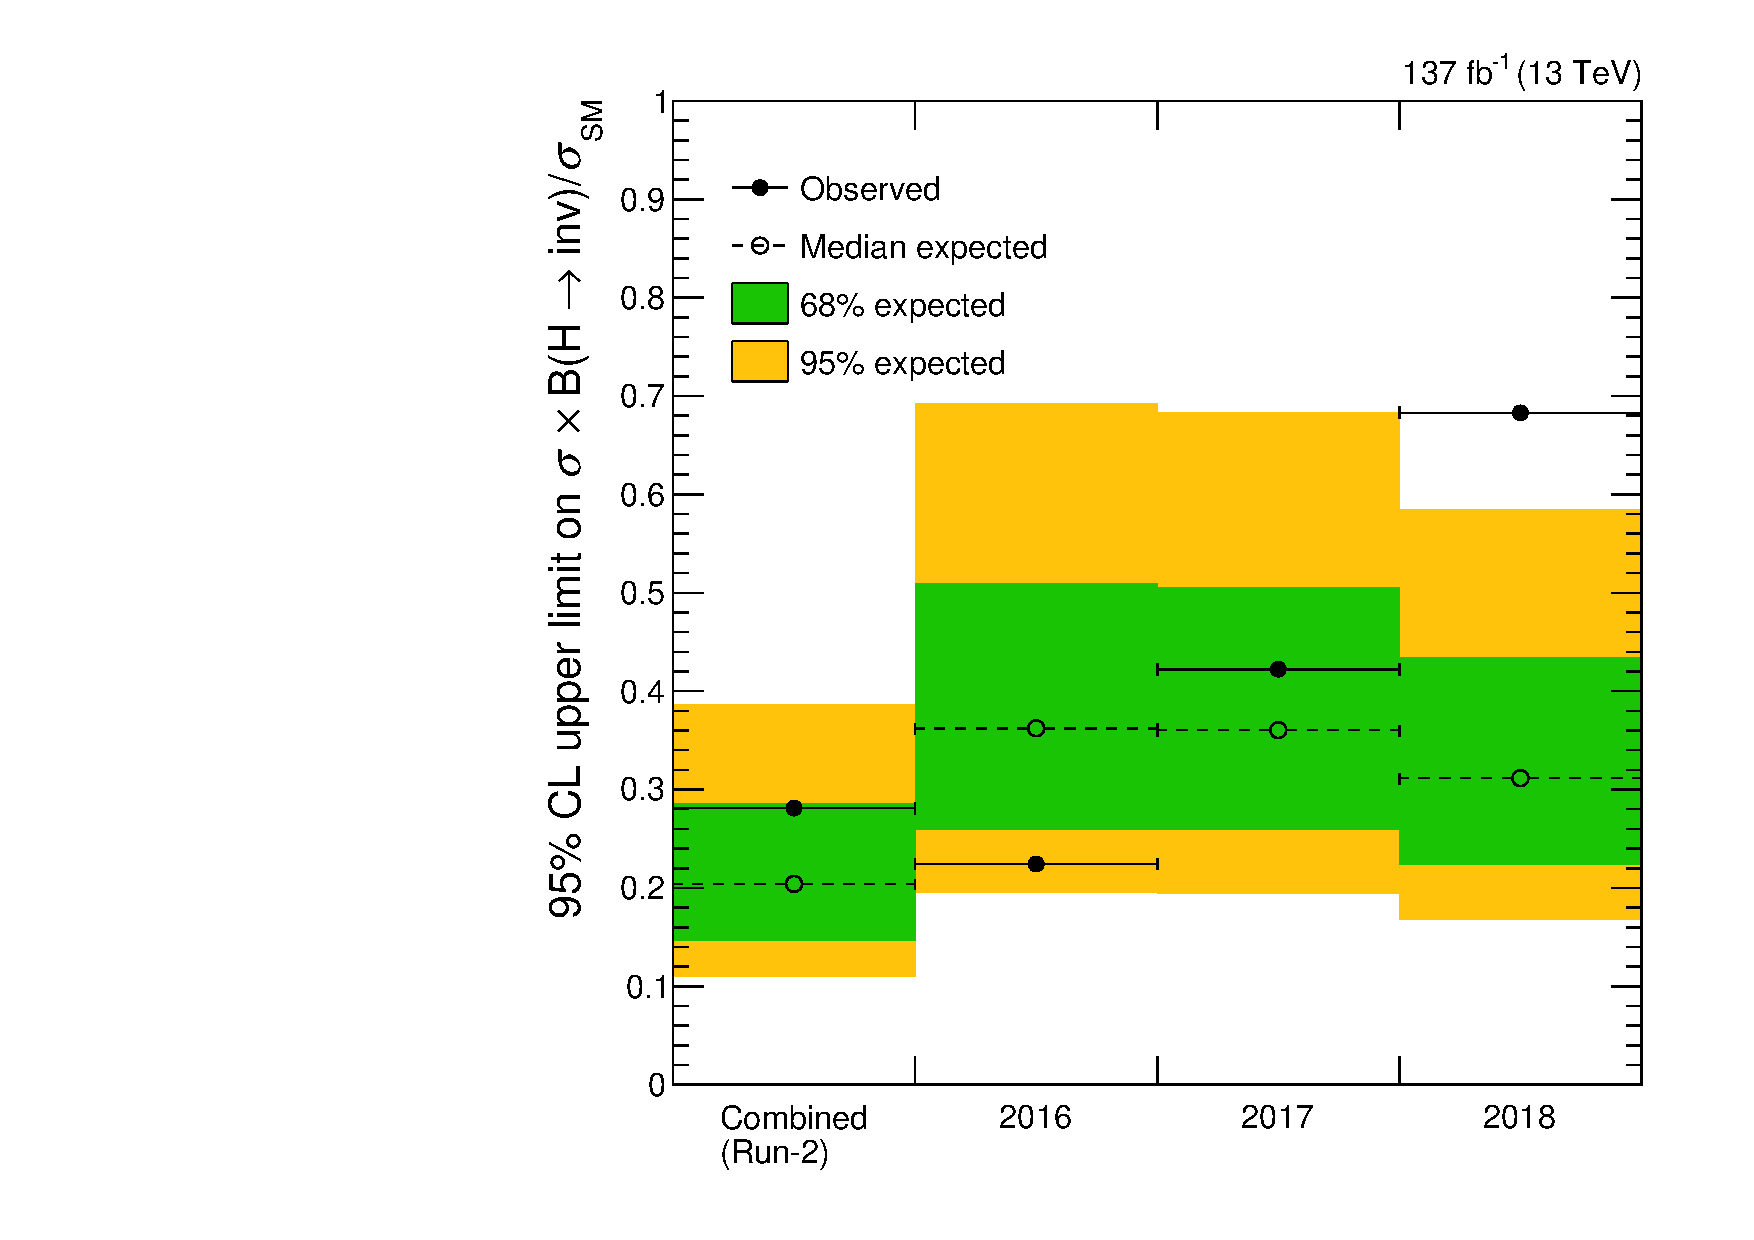
\includegraphics[width=\textwidth]{figures/limits/full_Run2/limit_Run2_comb_per_year.pdf}
        \caption{Limit --- Run-2}
    \end{subfigure}
    \hspace{0.05\textwidth}
    \begin{subfigure}[t]{0.45\textwidth}
        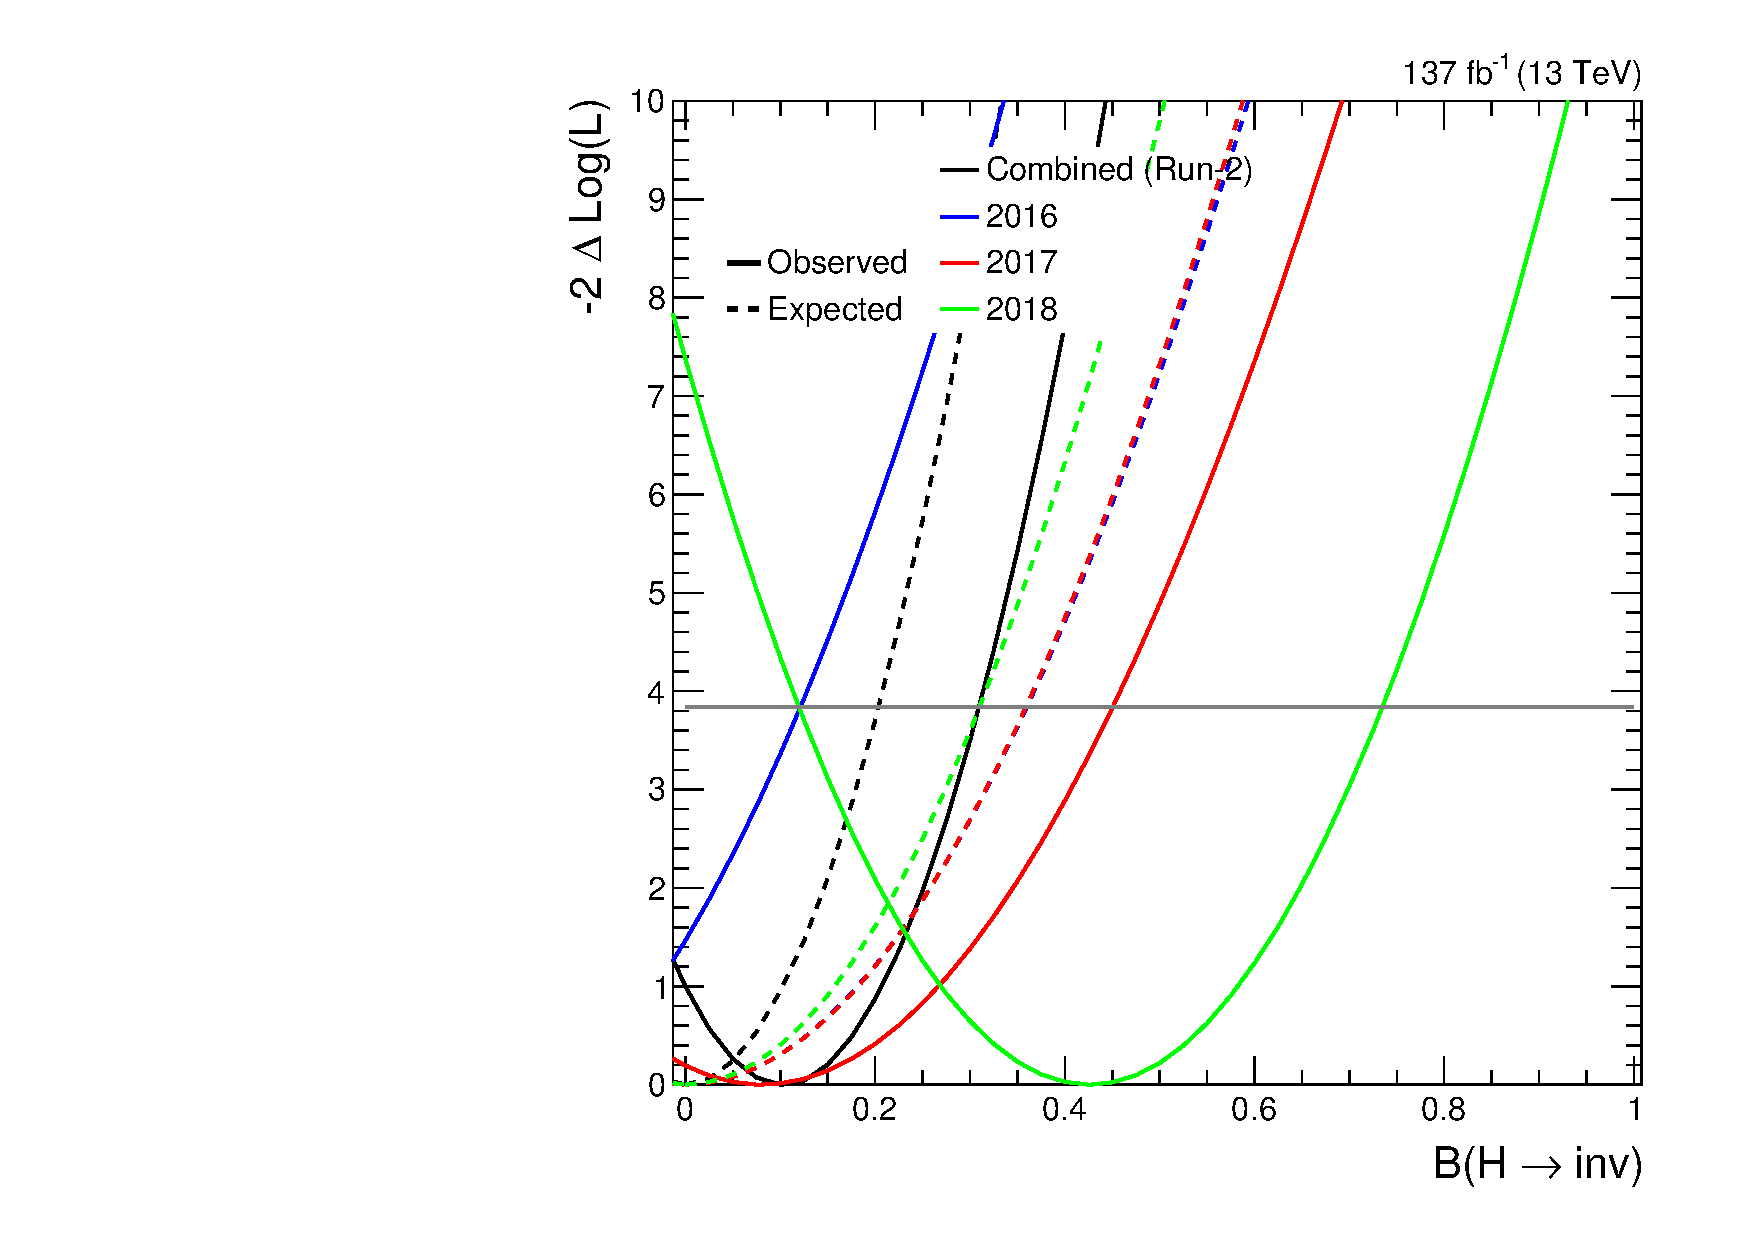
\includegraphics[width=\textwidth]{figures/likelihood_scan/profile_likelihood_scan_Run2_per_year.pdf}
        \caption{Profile likelihood --- Run-2}
    \end{subfigure}
    \caption[Observed and expected 95\,\% CL upper limit on the Higgs boson to invisible state branching fraction $\BRof{\higgstoinv}$ and the corresponding profile likelihood ratio as a function of it, for both the individual data taking years, as well as the combination of them, for the full Run-2 dataset]{Observed and expected 95\,\% CL upper limit on the Higgs boson to invisible state branching fraction $\BRof{\higgstoinv}$ (left) and the corresponding profile likelihood ratio as a function of it (right), for both the individual data taking years, as well as the combination of them, for the full Run-2 dataset. The \acrlong{sm} Higgs boson with its associated mass and production cross section are assumed.}
    \label{fig:htoinv_limit_likelihood_Run2_per_year}
\end{figure}

\begin{figure}[htbp]
    \centering
    \begin{subfigure}[t]{0.45\textwidth}  % top align since axis labels are larger for likelihood
        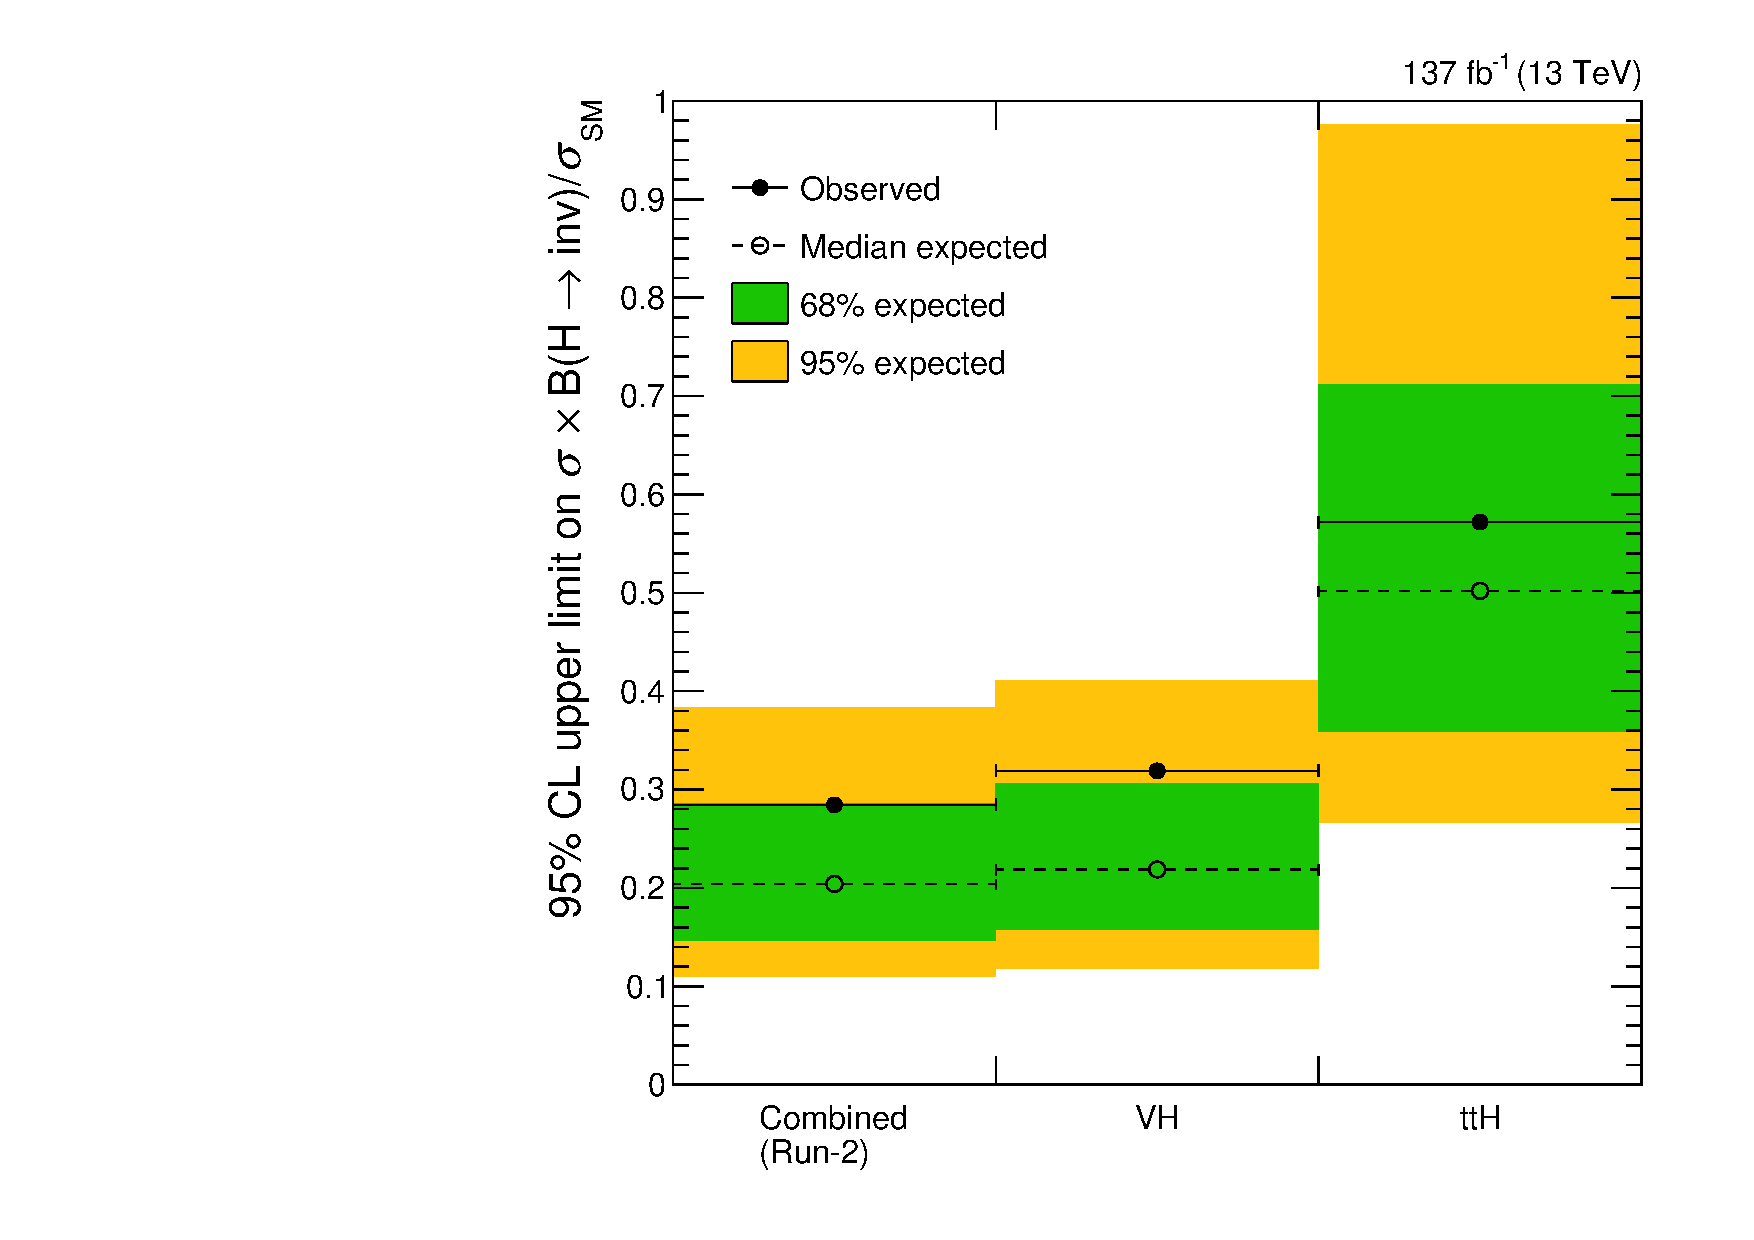
\includegraphics[width=\textwidth]{figures/limits/full_Run2/limit_Run2_comb_per_cat.pdf}
        \caption{Limit --- Run-2}
    \end{subfigure}
    \hspace{0.05\textwidth}
    \begin{subfigure}[t]{0.45\textwidth}
        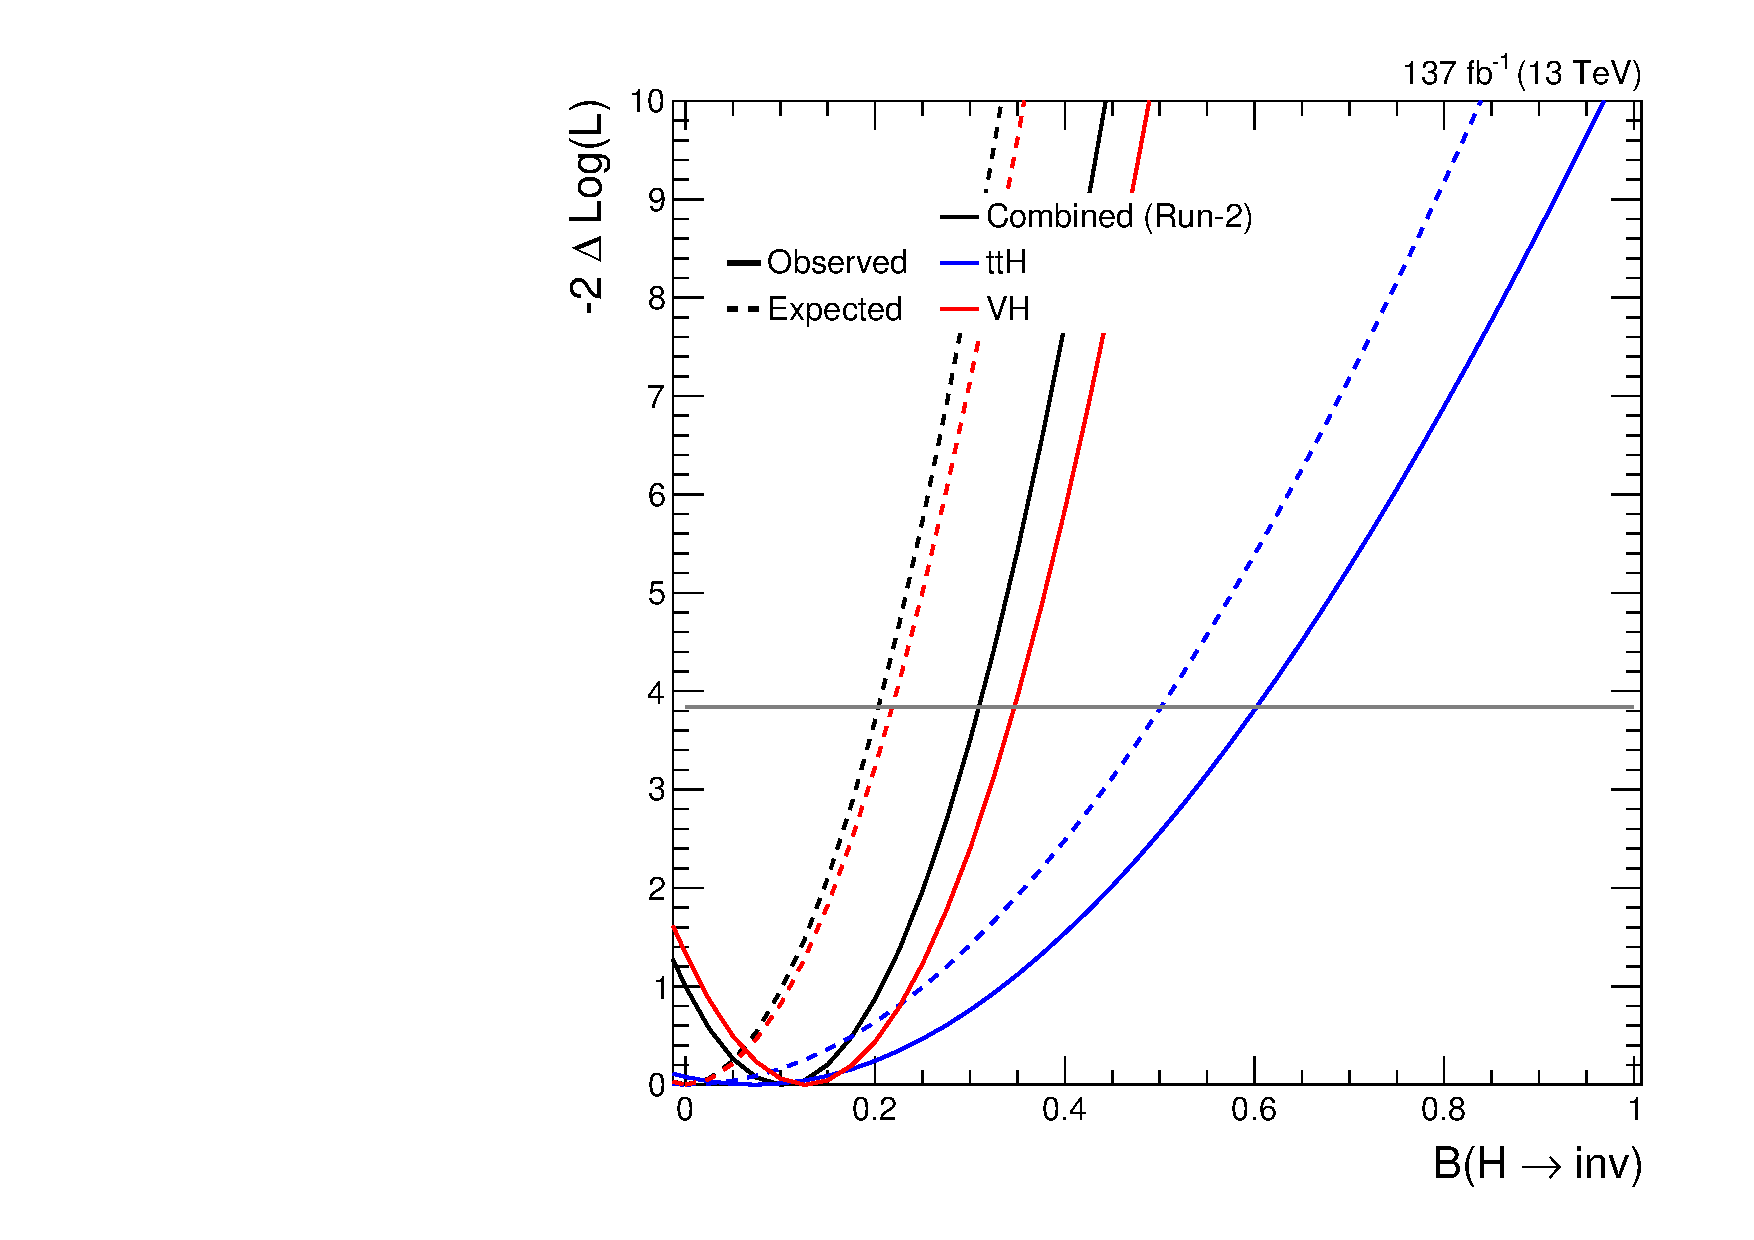
\includegraphics[width=\textwidth]{figures/likelihood_scan/profile_likelihood_scan_Run2_per_cat.pdf}
        \caption{Profile likelihood --- Run-2}
    \end{subfigure}
    \caption[Observed and expected 95\,\% CL upper limit on the Higgs boson to invisible state branching fraction $\BRof{\higgstoinv}$ and the corresponding profile likelihood ratio as a function of it, for both the individual categories, as well as the combination of them, for the full Run-2 dataset]{Observed and expected 95\,\% CL upper limit on the Higgs boson to invisible state branching fraction $\BRof{\higgstoinv}$ (left) and the corresponding profile likelihood ratio as a function of it (right), for both the individual categories, as well as the combination of them, for the full Run-2 dataset. The \acrlong{sm} Higgs boson with its associated mass and production cross section are assumed.}
    \label{fig:htoinv_limit_likelihood_Run2_per_cat}
\end{figure}

\begin{table}[htbp]
    \centering
    \begin{tabular}{ccccc}
        \hline\hline
        Dataset & \ttH & \VH & Combined\\\hline
        \multirow{2}{*}{2016} & 88\,\% (obs.) & 22\,\% (obs.) & 22\,\% (obs.) \\
        & 80\,\% (exp.) & 41\,\% (exp.) & 36\,\% (exp.) \\\hline
        \multirow{2}{*}{2017} & 115\,\% (obs.) & 43\,\% (obs.) & 42\,\% (obs.) \\
        & 90\,\% (exp.) & 38\,\% (exp.) & 36\,\% (exp.) \\\hline
        \multirow{2}{*}{2018} & 96\,\% (obs.) & 73\,\% (obs.) & 68\,\% (obs.) \\
        & 80\,\% (exp.) & 34\,\% (exp.) & 31\,\% (exp.) \\\hline
        \multirow{2}{*}{Run-2} & 56\,\% (obs.) & 32\,\% (obs.) & \textbf{28\,\% (obs.)} \\
        & 50\,\% (exp.) & 22\,\% (exp.) & \textbf{20\,\% (exp.)} \\\hline\hline
    \end{tabular}
    \caption[Observed and median expected upper limits on $\BRof{\higgstoinv}$ at 95\,\% confidence level for each combination of category and dataset in the analysis]{Observed and median expected upper limits on $\BRof{\higgstoinv}$ at 95\,\% confidence level for each combination of category and dataset in the analysis.}
    \label{tab:hinv_limits}
\end{table}
